\chapter{Problem Definition}
\label{problem}

The primary objective of this project is to implement a \textit{multi-purpose recommender framework} to overcome specific issues of recommender systems explained further in this section. The focus on \emph{framework} intends to emphasise an ecosystem which provides a distinctive tool kit to build multiple recommender systems, yet guarantees a simple integration. Insofar the focus of the project will be in the design of an alternative -- perhaps novel -- architecture rather than in the details of techniques and algorithms.

This section discusses the requirements of the proposed framework while pointing to aforementioned issues of recommender systems. The requirements \emph{interoperability}, \emph{abstraction}, \emph{ease of integration} and \emph{service-orientation} will become measures on how successful the proposed solution is in overcoming those issues.

Finally, existing research as well as solutions are examined in their coping with those challenges.



\section{Framework Requirements}

\subsection{Multipurpose \& Interoperability}
\label{problem-multipurpose}

A \emph{multi-purpose} recommender system is able to cope with different data sources and techniques. Ideally this system is open and extendable for possible forthcoming, yet unknown requirements. It is not to be confused with hybrid recommender systems (see section \ref{bg-tech-hybrid}) which combine different systems into one. In this project I will provide an ecosystem to plug different recommender systems in (see section \ref{sol-design-layer-reco}).

Another requirement is the interoperability between recommender systems. \citet{manouselis07} differentiate between three criteria:

\begin{description}
    \item[Interoperability of the recommendation queries] which allows the same query to be reused. This is in particular useful for hybrid recommender systems which feeds the same query into different systems. \citet{adomavicius05} go further and creates a \emph{Recommendation Query Language (RQL)}. The use of an RQL would go beyond the scope of this project. Therefore I will limit this criterion to query parameters rather than the full query and rely on the recommender system to build the query based on these parameters. To give an example, the query parameters for figure \ref{fig:contentbased} would be the customer reference and the rated item (in this case the laptop). A content-based recommender system would compute these parameters by looking up similar items whereas a collaborative filtering system would look for other users who rated this item.
    \item[Interoperability of the user and the domain models] which allows the exchange of models and other data among different recommender systems. In this project I will go a step further and allow direct access to persistence layers to all recommender systems.
    \item[Interoperability of the recommendation results] which empowers recommender systems to reuse the results. This is in particular useful for hybrid recommender systems which feeds the same query into different systems. Yet there is no use casein this project and therefore not covered.
\end{description}

\subsection{Abstraction}
\label{problem-abstraction}

Recommender systems are usually tightly coupled to the primary application, which is the main application using the recommender system. \citet{cortizo10} claim that recommender systems are designed for a specific data structure. This comes with the following challenges:

\begin{description}

    \item[Complexity] Applications as well as recommender systems tend to be complex. If not separated they both add to the overall complexity which makes change management very difficult, time consuming and expensive. Any change requires knowledge -- higher human resources costs --, testing and probably modifications on both systems. Figure \ref{fig:abstraction-complexity} shows a tightly coupled system whose one recommender system is getting replaced. The whole primary application as well as the database are getting affected.

    \begin{figure}[H]
        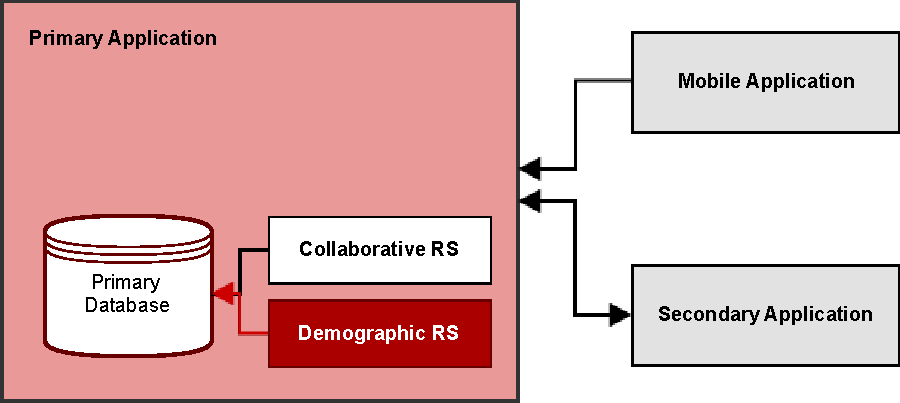
\includegraphics[width=0.7\textwidth,center]{problem/abstraction/complexity.pdf}
        \caption{Abstraction: Complexity}
        \label{fig:abstraction-complexity}
    \end{figure}

    \item[Database Abstraction] Recommender systems directly using databases of the primary or other applications are problematic as on one hand they are affected to any schema changes done to the database due to application modifications. Figure \ref{fig:abstraction-database} illustrates a semi-decoupled architecture where the recommender system is outside of the primary application, yet still uses its database. This gives a false impression of loose coupling. Teams working on the primary application might not fully aware that there changes affect other systems.

    \begin{figure}[H]
        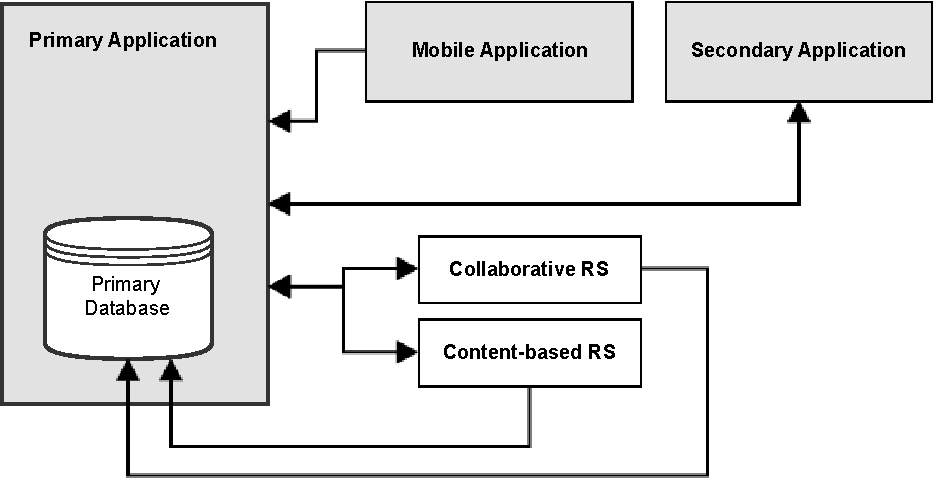
\includegraphics[width=0.7\textwidth,center]{problem/abstraction/database.pdf}
        \caption{Abstraction: Missing Database Abstraction}
        \label{fig:abstraction-database}
    \end{figure}

    \item[Reusability] Tightly coupled components are difficult to reuse. Figure \ref{fig:abstraction-resuability} shows an architecture where other applications and even devices such as mobile can reuse the recommender systems.

    \begin{figure}[H]
        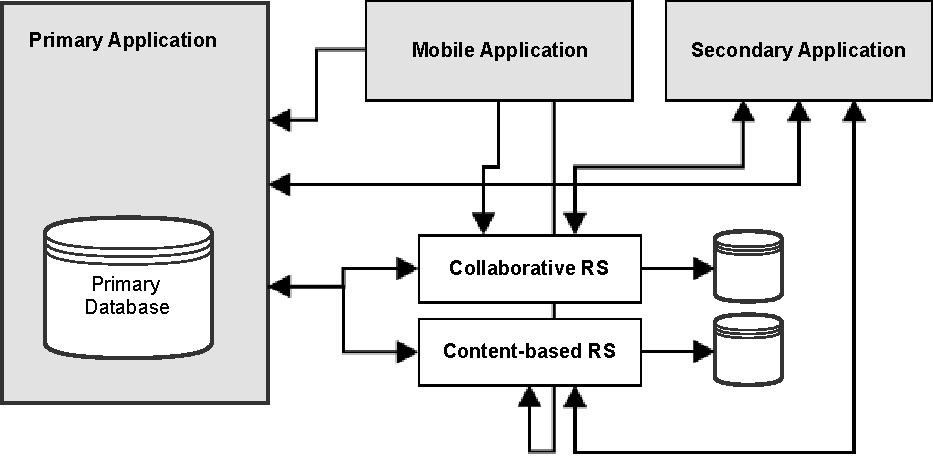
\includegraphics[width=0.7\textwidth,center]{problem/abstraction/reusability.pdf}
        \caption{Abstraction: Reusable Architecture}
        \label{fig:abstraction-resuability}
    \end{figure}

    \item[Dependancy] If a system needs to be replaced or modified, it can have more or less major implications to other systems depending on that system. Figure \ref{fig:abstraction-dependancy} shows a loosely coupled architecture where the recommender technique has been changed from content-based to demographic filtering. Due to the loose coupling it has less implications than in figure \ref{fig:abstraction-complexity}. However it can still affect other systems if the communication between them included content-based filtering specific logic.

    \begin{figure}[H]
        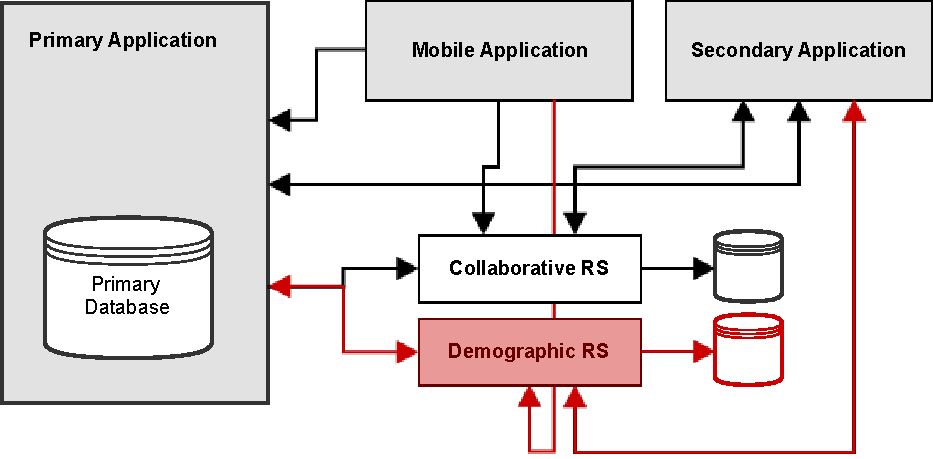
\includegraphics[width=0.7\textwidth,center]{problem/abstraction/dependancy.pdf}
        \caption{Abstraction: Dependancy Issues}
        \label{fig:abstraction-dependancy}
    \end{figure}

    \item[Encapsulation] Information hiding is the fundamental motivation for encapsulation. The more information and implementation is hidden, the looser the coupling becomes. Figure \ref{fig:abstraction-encapsulation} illustrates a recommender system framework which hides internal details and communicates with other components in an implementation unspecific manner. A change of a technique within the framework or an external application should not have any implications.

    \begin{figure}[H]
        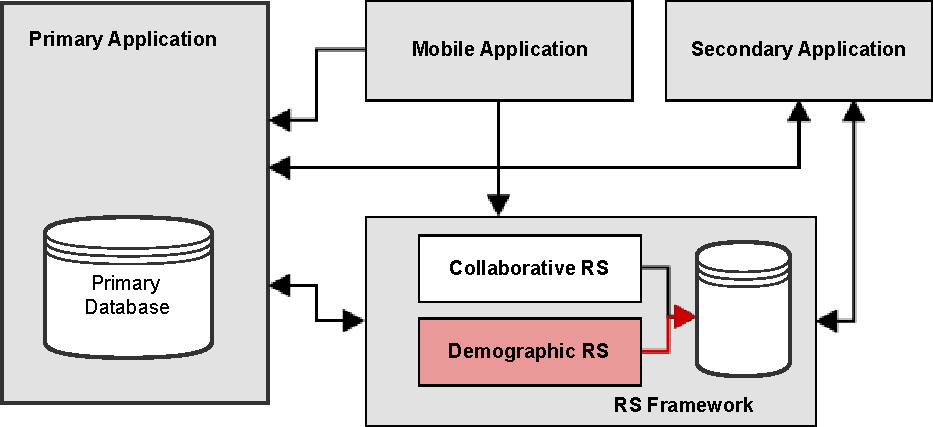
\includegraphics[width=0.7\textwidth,center]{problem/abstraction/encapsulation.pdf}
        \caption{Abstraction: Encapsulation}
        \label{fig:abstraction-encapsulation}
    \end{figure}
\end{description}

\subsection{Ease of Integration}

The complexity and cost of integrating recommender systems is a major constraint for many projects. Given the requirements above it is even more challenging to keep the integration as easy as possible. Nonetheless abstraction should help reduce the amount of knowledge needed. Furthermore the fewer types of communication and configuration required the less effort will be necessary.



\section{Evaluation of Existing Research and Solutions}
\label{prob-evaluation}

As mentioned in \ref{bg-adoption}, recommender systems are considered a relatively new research area in computer science. Although it has gained attention recently, a considerable amount of research has been published on the fundamental concepts and techniques rather than on matters of integration and architecture. Nonetheless I found that \citet{cortizo10} and \citet{rack07} worked on similar approaches.

\citet{cortizo10} built a \textit{general purpose multi-algorithm} recommender system to compute recommendations from different sources and serving multiple applications. They mention that they could not find any literature on the system's aspects of recommender systems. \citet{cortizo10} identified similar challenges and made similar decisions on the implementation especially using RESTful APIs (see section \ref{sol-design-layer}). The advantage of their work was that they evaluated and tested their system on a live environment. Scalability and performance were key metrics from the beginning. Their recommender system is not open source and therefore not available for me.

\citet{rack07} have published a series of papers around their work on the \emph{AMAYA} recommender system. Although they have put an emphasis on multi-purposeness, their work is more oriented towards a context-aware recommender system which differentiates between contexts such as \emph{'being home'} and \emph{'being at work'}. Furthermore their recommender requires a user profile as a centre point. In summary, their architecture is not as flexible and unbiased as the design I propose. The last submitted paper about \emph{AMAYA} was in 2007 and the system is again not publicly available.

There are several commercial recommender software available such as \emph{prudsys Realtime Decisioning Engine (RDE)} which I have integrated into a major e-commerce website in the past. In a brief analysis of commercial software I found that they usually cover only basic but common requirements for e-commerce websites. These products are closed source and therefore not beneficial for my project. 

\citet{hahsler11} and \citet{rack07} provide a list of open source recommender systems which are freely available. In the majority these systems are more component libraries than complete solutions. They require significant amount of work to integrate. Amongst them is \emph{Apache Mahout} -- a machine learning library which also includes collaborative filtering components. \emph{Mahout} is built upon \emph{Hadoop} which is a well-established big data software also curated by \emph{The Apache Software Foundation}. \emph{easyrec} on the other hand is a complete solution which is also using RESTful APIs. However -- similar to commercial products -- it is opiniated in favor of e-commerce websites.